\chapter{Metodi} % (fold)
\label{cha:Metodi}

Tutti i dati sono stati raccolti da analisi ecografiche effettuate presso l'\textbf{Azienda
	Ospedaliera Universitaria di Parma}, nel periodo tra \textbf{Aprile 2022} e \textbf{Gennaio 2023} da
un team di medici. Per standardizzare le immagini raccolte, sono stati applicati i
seguenti parametri per la standardizzazione dell'immagine:

\begin{itemize}
	\item Indice di massa corporea (BMI)
	\item Età
	\item Problematiche durante la gravidanza
	\item Problematiche dopo la gravidanza
	\item Femore centrato nell'inquadratura
\end{itemize}

Le immagini hanno subito un processo di \textit{preprocessing} aggiuntivo per
uniformare le dimensioni e la risoluzione. In particolare, sono state
ridimensionate a immagini \textbf{$1280px$ di larghezza} e \textbf{$876px$ di
	altezza}.

Inoltre data la tipologia del problema, si è scelto di convertire le immagine da
\textbf{RGB} a immagini in \textbf{scala di grigi} per ridurre la complessità del problema
e per ridurre il quantitativo di dati necessari per l'addestramento della rete.

Sono state realizzate manualmente delle \textbf{maschere} di segmentazione per
ogni immagine, in modo da avere un \textit{ground truth} da confrontare con le
predizioni del modello.

Data la scarsa quanti di dati a disposizione per l'addestramento della U-Net, si è scelto
di utilizzare alcune tecniche di \textit{data augmentation} per aumentare la quantità di
dati a disposizione. In particolare si è scelto di utilizzare le seguenti tecniche
applicate in modo casuale per ogni coppia \textbf{immagine-maschera}
\begin{itemize}
	\item \textit{Flip} orizzontale e verticale
	\item \textit{Rotazioni} di $35^{\circ}$
	\item \textit{Rumore} Gaussiano
\end{itemize}

Queste tecniche hanno migliorato notevolmente le segmentazioni ottenute tramite la rete U-Net,
aumentando la robustezza della rete alle variazioni di luce e al rumore nelle immagini.

\begin{figure}[!ht]
	\centering
	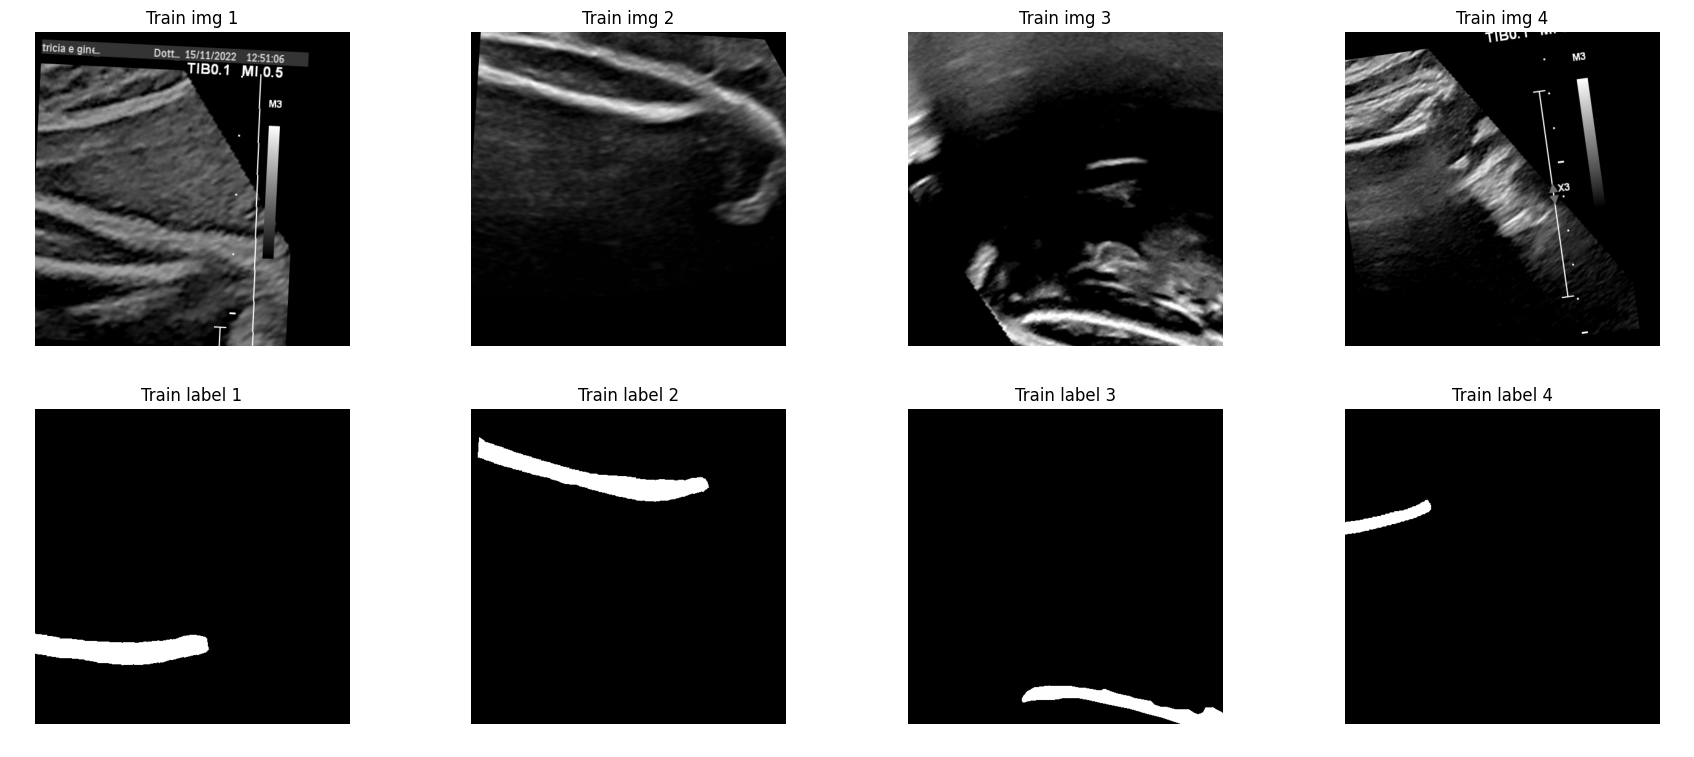
\includegraphics[width=0.8\textwidth]{Immagini/data_augmentation_train.png}
	\caption{Immagini utilizzate per l'addestramento}
	\label{fig:data_augmentation_train}
\end{figure}

L'efficacia della \textit{data augmentation} nella fase di addestramento del modello è evidente,
migliorando l'adattabilità a contesti non controllati e la generalizzazione del modello. Come
mostrato in \autoref{fig:data_augmentation_train}, la \textit{data augmentation} è stata applicata in modo
casuale per ogni coppia \textbf{immagine-maschera}.

Soltanto le immagini utilizzate per l'addestramento sono state sottoposte a \textit{data augmentation},
le immagini contenute nel \textit{test set} e nel \textit{validation set} sono rimaste invariate.


\begin{figure}[!ht]
	\centering
	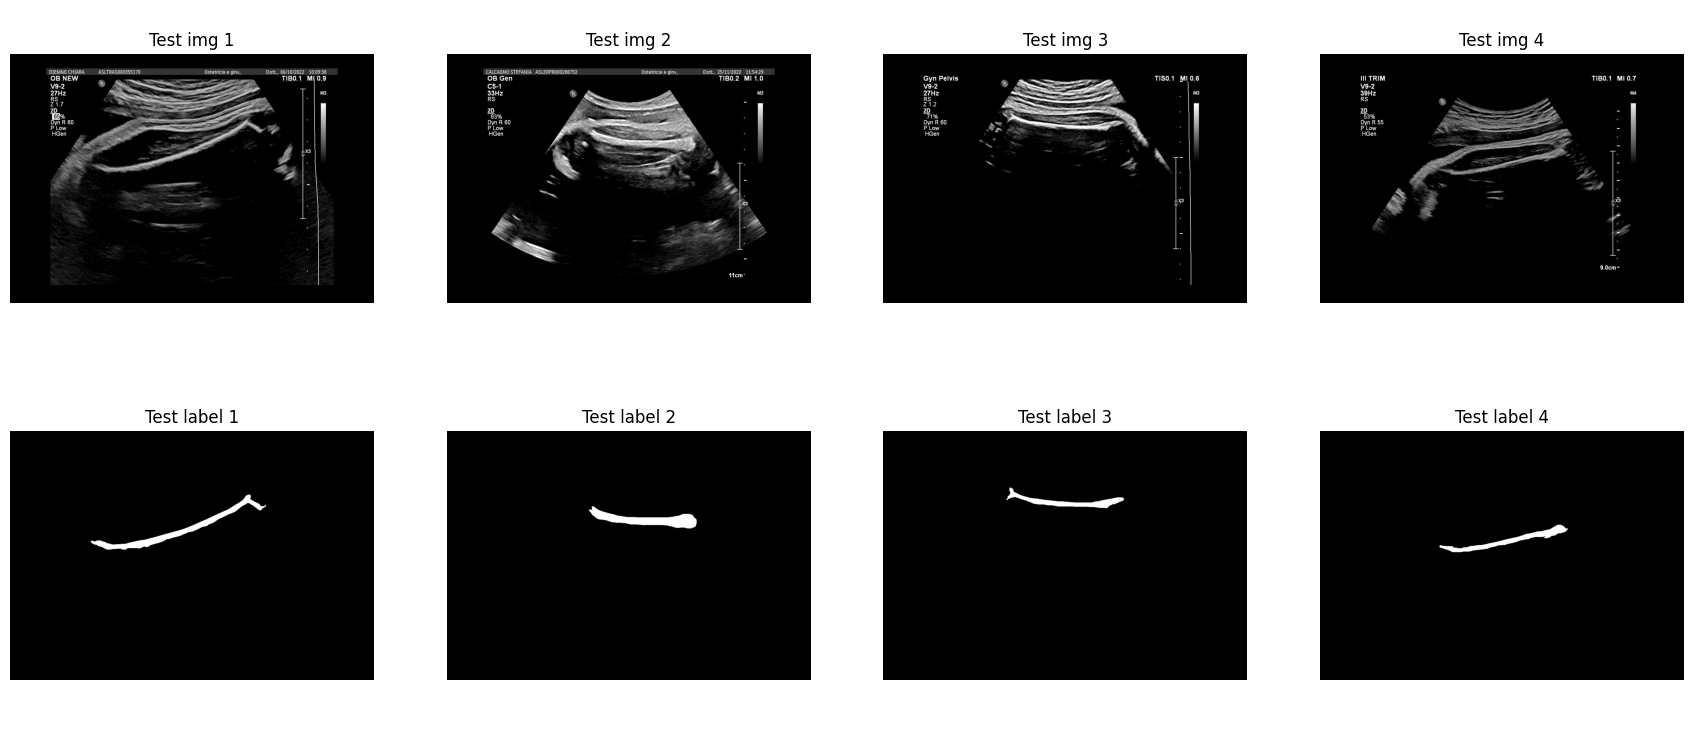
\includegraphics[width=0.8\textwidth]{Immagini/data_augmentation_test.png}
	\caption{Immagini utilizzate nel test set}
	\label{fig:data_augmentation_test}
\end{figure}

\begin{figure}[!ht]
	\centering
	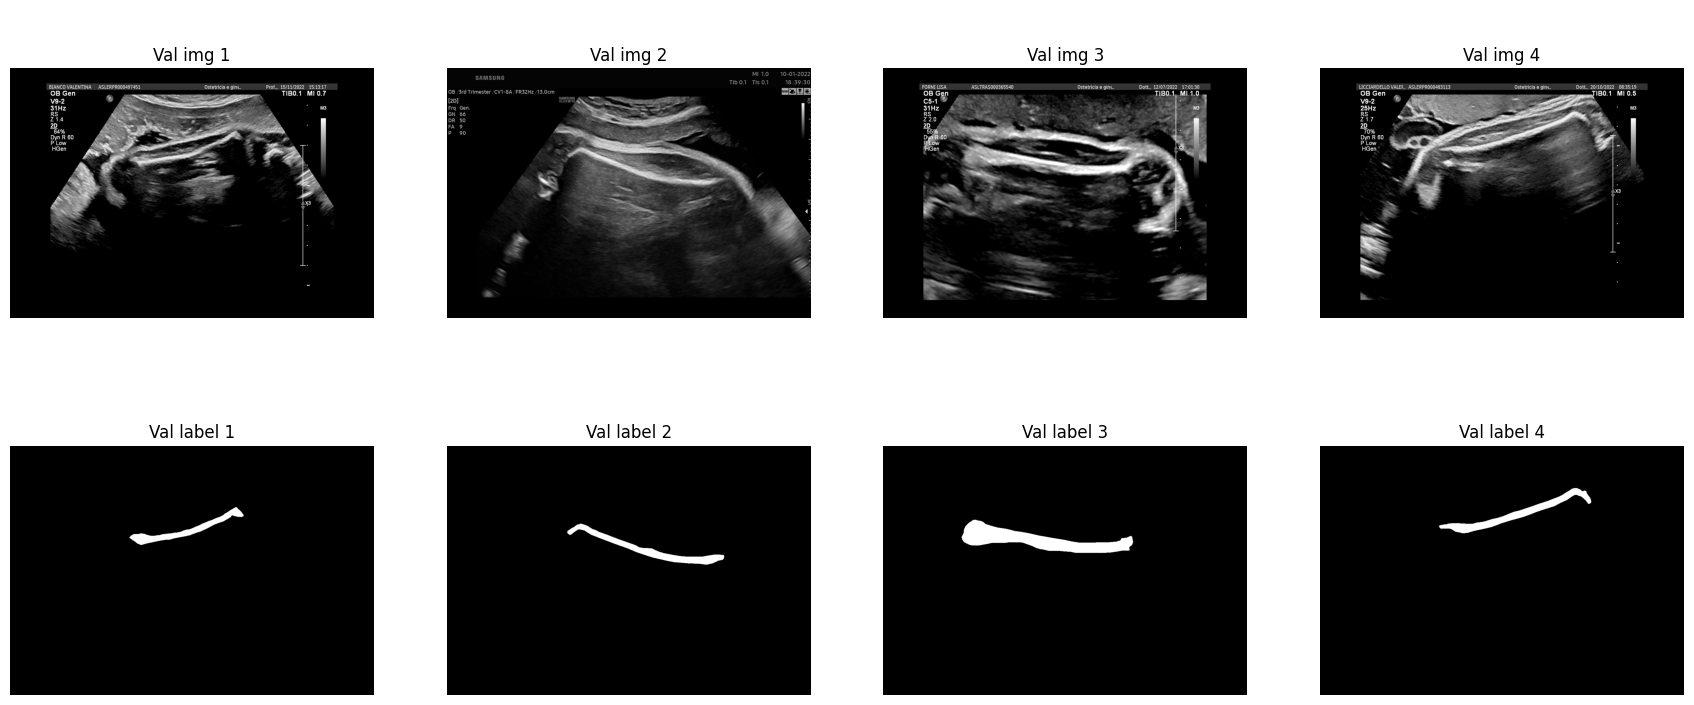
\includegraphics[width=0.8\textwidth]{Immagini/data_augmentation_val.png}
	\caption{Immagini utilizzate nel validation set}
	\label{fig:data_augmentation_val}
\end{figure}

È fondamentale che i set di test e validazione riflettano accuratamente le condizioni reali di
utilizzo, per valutare efficacemente le prestazioni del modello. L'introduzione di variazioni
artificiali tramite data augmentation in questi set potrebbe portare a una valutazione distorta
delle capacità del modello.

Mentre la data augmentation durante l'addestramento espone la rete a una varietà maggiore di dati, è
essenziale valutare la rete su dati non alterati per assicurarsi che abbia imparato a generalizzare
correttamente.



\section{Etichettatura}
Le immagini utilizzate per l'addestramento della rete sono state etichettate manualmente utilizzando
un software di etichettatura chiamato \textbf{LabelMe} \cite{labelme}.

Il processo di etichettatura comporta la selezione accurata e la delimitazione del perimetro del
femore in ciascuna immagine. Sono applicato indicatori specifici attorno alla regione di interesse,
in modo da isolare il femore dal resto dell'immagine. Questo approccio di etichettatura mirata è
cruciale per fornire alla rete neurale esempi precisi da cui imparare, migliorando così la sua
capacità di identificare correttamente le strutture anatomiche nelle immagini.

La corretta etichettatura è vitale non solo per l'addestramento efficace della rete, ma anche per
garantire l'affidabilità e l'accuratezza delle segmentazioni future. Essa permette alla rete di
riconoscere le variazioni sottili e le caratteristiche specifiche del femore, che sono essenziali
per applicazioni mediche precise e affidabili.




\section{Modello}

Il modello scelto come punto di partenza per questo studio è il \textbf{U-Net} (\autoref{fig:unet}),
la cui architettura originale è stata sviluppata da Olaf Ronneberger, Philipp Fischer e Thomas Brox
nel 2015 \cite{ronneberger2015unet}. Questo studio propone un'architettura di rete neurale
convoluzionale specificamente progettata per la segmentazione semantica di immagini biomediche, in
cui ogni singolo pixel dell'immagine è classificato in una delle categorie pertinenti al problema
analizzato.

Lo studio propone un'architettura di rete neurale convoluzionale per la
segmentazione semantica di immagini biomediche, classificando ogni singolo pixel
dell'immagine in una delle varie categorie del problema analizzato, la rete
convoluzionale emersa da questa analisi rimane tutto' oggi una delle più
utilizzate in ambito medico per la segmentazione semantica data la sue
performance e la sua versatilità.

L'implementazione iniziale ricalca il modello realizzato da Olaf Ronneberger,
Philipp Fischer e Thomas Brox, utilizzando il framework \textbf{PyTorch}
\cite{pytorch} come base per la realizzazione della rete.


\section{Architettura U-Net}

L'architettura proposta da Olaf Ronneberger, Philipp Fischer e Thomas Brox è
composta di 4 parti principali:
\begin{itemize}
	\item \textbf{Encoder}:
	      Visionabile graficamente come la parte discendente della U-Net
	\item \textbf{Bridge}: Visionabile graficamente come la linea di congiunzione fra la
	      parte discendente e la parte ascendente della U-Net
	\item \textbf{Decoder}: Visionabile graficamente come la parte ascendente della U-Net
	\item \textbf{Output}: Visionabile graficamente come l'ultimo layer della U-Net
\end{itemize}

Le applicazioni che si appoggiano a modelli derivati dall'architettura U-net
dominano settori come la medicina e la biologia, in particolare la segmentazione
di immagini biomediche, come la segmentazione di immagini ecografiche, la
segmentazione di immagini TC e la segmentazione di immagini RM.

I motivi principali del successo di U-Net includono:
\begin{itemize}
	\item \textbf{Segmentazione dettagliata}: U-Net è capace di produrre segmentazioni dettagliate e
	      precise grazie alle sue innovative "skip connections", che consentono al modello di
	      catturare sia i dettagli di basso livello che il contesto di alto livello.
	\item \textbf{Architettura compatta}: Nonostante la sua elevata capacità di dettaglio, il
	      modello rimane relativamente snello e può essere addestrato con successo anche con dataset
	      di dimensioni moderate.
	\item \textbf{Adattabilità}: Originariamente concepita per applicazioni mediche, U-Net ha
	      dimostrato un'elevata versatilità, adattandosi a una vasta gamma di applicazioni.
\end{itemize}

Tuttavia, come ogni modello, U-Net presenta anche alcuni svantaggi. Il principale riguarda la
necessità di un dataset di addestramento ampio e accuratamente etichettato, che può essere un
ostacolo in contesti con dati limitati. Inoltre, U-Net richiede una quantità significativa di
memoria per memorizzare i pesi del modello, il che può rappresentare un problema nel caso di
immagini ad alta risoluzione.


\subsection{Convoluzione}
\label{sec:convoluzione}

La convoluzione è una delle operazioni fondamentali utilizzate nelle reti
neurali convoluzionali per estrarre le caratteristiche significative da un'
input, la convoluzione coinvolge un filtro (o kernel) e l'input su cui si
applica.

Il processo di convoluzione consiste nel sommare ogni elemento di un'immagine
al suo vicino, pesando ogni singola operazione mediante l'utilizzo del filtro(o
kernel) il calcolo della feature map di uscita è calcolata come segue:
\begin{align}
	 & \Bigg( \begin{bmatrix}
		          a & b & c \\
		          d & e & f \\
		          g & h & i
	          \end{bmatrix}
	*
	\begin{bmatrix}
		1 & 2 & 3 \\
		4 & 5 & 6 \\
		7 & 8 & 9
	\end{bmatrix}
	\Bigg) [2, 2] =                                                                                                                  \\
	 & = (i \cdot 1) + (h \cdot 2) + (g \cdot 3) + (f \cdot 4) + (e \cdot 5) + (d \cdot 6) + (c \cdot 7) + (b \cdot 8) + (a \cdot 9)
\end{align}


\subsection{Max Pooling}
\label{sec:max_pooling}

Il \textit{max pooling} è un'operazione chiave all'interno delle reti neurali convoluzionali (CNN),
inclusa la rete U-Net.

Il \textit{max pooling} è utilizzato per ridurre la dimensione delle feature
map, consentendo di ridurre la complessità del problema da approssimare,
comportando una maggior resistenza al \textit{overfitting}, migliorando la
capacit\'a di generalizzazione del modello e di ottenere una rappresentazione
più invariante rispetto alle piccole variazioni spaziali nell'input.


\subsection{Encoder}
\label{sec:Encoder}

La fase di \textit{encoding} rappresenta la prima parte della rete U-Net, ed è composta da una serie
di strati di convoluzione (vedi Sezione \ref{sec:convoluzione}) e max pooling (vedi Sezione
\ref{sec:max_pooling}). Questi strati lavorano per ridurre progressivamente la dimensione spaziale
dell'immagine, aumentando contemporaneamente il numero di canali delle \textit{features}.

Nello specifico, la fase di \textit{encoding} comprende tre componenti principali:
\begin{itemize}
	\item \textbf{Strato iniziale}: Questo strato applica diverse operazioni di convoluzione ai dati
	      di input per estrarre caratteristiche di basso livello, come bordi e texture.
	\item \textbf{Downsampling}: Successivamente, si utilizzano operazioni di max pooling o
	      convoluzione con un passo (stride) superiore a 1 per ridurre la dimensione delle feature map.
	\item \textbf{Strati intermedi}: Questi strati applicano ulteriori operazioni di convoluzione per
	      catturare caratteristiche di complessità crescente.
\end{itemize}


\subsection{Decoder}
\label{sec:Decoder}

La fase di \textit{decoding} nella rete U-Net è incaricata di ricostruire l'immagine segmentata a
partire dalle informazioni estratte durante la fase di \textit{encoding}. Le fasi principali del
decoder includono:
\begin{itemize}
	\item \textbf{Upsampling}: La fase di decoding inizia con l'operazione di upsampling, che serve a ripristinare gradualmente la dimensione delle feature map ai livelli originali dell'immagine. Ciò viene fatto utilizzando operazioni come la trasposta della convoluzione (de convoluzione) o l'interpolazione bilineare. L'obiettivo è ottenere feature map di dimensioni compatibili con quelle dell'immagine di input.
	\item \textbf{Skip Connections}: Un aspetto distintivo della U-Net sono le skip connections, o connessioni di salto. Queste connessioni collegano le feature map estratte durante l' encoding alle corrispondenti feature map nella fase di decoding. Ciò consente di combinare informazioni multi-scala, in modo che il modello possa accedere sia a dettagli fini che a contesto di alto livello. Le skip connections sono fondamentali per migliorare la precisione della segmentazione.
	\item \textbf{Convoluzione nel Decoding}: Dopo l' upsampling e l'integrazione delle skip connections, vengono applicate operazioni di convoluzione per raffinare ulteriormente le feature map. Queste convoluzioni possono avere lo scopo di "mescolare" le informazioni o di catturare dettagli specifici a livelli più alti.
\end{itemize}

\subsection{Bridge}
\label{sec:Bridge}

Il \textit{bridge} è una componente cruciale dell'architettura U-Net, che facilita il trasferimento
di informazioni rilevanti tra l'encoder e il decoder attraverso le \textit{skip connections}. Questa fase
consente di considerare dettagli sia di basso che di alto livello durante il processo di
segmentazione.

\subsection{Output}
\label{sec:Output}
La parte finale della rete U-Net è costituita da uno o più strati di convoluzione che riducono la
profondità delle feature map alla dimensione richiesta per l'output finale, producendo così
l'immagine segmentata.


\section{Rimozione della Sliding Window}
\label{sub:Rimozione sliding window}

Con gli avanzamenti tecnologici nel campo dell'hardware e del software, si è osservato un notevole
miglioramento nei tempi di elaborazione delle immagini e nella capacità di gestire immagini di
grandi dimensioni. Pertanto, si è deciso di abbandonare l'approccio della sliding window, che è più
conservativo in termini di utilizzo della memoria e tempo di elaborazione.

Al suo posto, si è adottato un metodo più moderno che sfrutta la potenza di calcolo delle GPU
attuali e la loro memoria dedicata, significativamente più ampia rispetto alle generazioni
precedenti. L'utilizzo di immagini complete, anziché porzioni separate tramite sliding window, ha
prodotto un "effetto collaterale" positivo: una migliore comprensione spaziale delle immagini da
parte della rete.

La visualizzazione dell'intera immagine consente alla rete di acquisire una migliore comprensione
del contesto spaziale, migliorando così la precisione della segmentazione.


\section{Modifica della Struttura Encoder-Decoder}
\label{sub:Modifica Encoder-Decoder}

Durante le fasi sperimentali, è emerso che aumentando il numero di iterazioni di convoluzione nei
vari strati di encoding e decoding si ottengono risultati migliori in termini di segmentazione.
Questo miglioramento, tuttavia, comporta un aumento del tempo di elaborazione e del consumo di
memoria.

Di conseguenza, si è deciso di modificare le fasi di \textit{encoding} e \textit{decoding} come segue:

\begin{table}[!ht]
	\centering
	\begin{tabular}{|c|c|c|}
		\hline
		\textbf{Layer} & \textbf{In channels} & \textbf{Out channels} \\
		\hline
		\hline
		Encoder        & 1                    & 64                    \\
		\hline
		Encoder        & 64                   & 128                   \\
		\hline
		Encoder        & 128                  & 256                   \\
		\hline
		Encoder        & 256                  & 512                   \\
		\hline
		Decoder        & 1024                 & 512                   \\
		\hline
		Decoder        & 512                  & 256                   \\
		\hline
		Decoder        & 256                  & 128                   \\
		\hline
		Decoder        & 128                  & 64                    \\
		\hline
	\end{tabular}
	\caption{Encoding e Decoding originali}
	\label{tab:encoding_originale}
\end{table}

\begin{table}[!ht]
	\centering
	\begin{tabular}{|c|c|c|}
		\hline
		\textbf{Layer} & \textbf{In channels} & \textbf{Out channels} \\
		\hline
		\hline
		Encoder        & 1                    & 16                    \\
		\hline
		Encoder        & 16                   & 32                    \\
		\hline
		Encoder        & 32                   & 64                    \\
		\hline
		Encoder        & 64                   & 128                   \\
		\hline
		Encoder        & 128                  & 256                   \\
		\hline
		Encoder        & 256                  & 512                   \\
		\hline
		Decoder        & 1024                 & 512                   \\
		\hline
		Decoder        & 512                  & 256                   \\
		\hline
		Decoder        & 256                  & 128                   \\
		\hline
		Decoder        & 128                  & 64                    \\
		\hline
		Decoder        & 64                   & 32                    \\
		\hline
		Decoder        & 32                   & 16                    \\
		\hline
	\end{tabular}
	\caption{Encoding e Decoding modificati}
	\label{tab:encoding_modificato}
\end{table}

L'intento di questa modifica è sfruttare la capacità di estrazione di feature delle operazioni di
convoluzione e di riduzione delle feature meno rilevanti tramite max pooling. Aggiungendo iterazioni
di convoluzioni, la rete può estrarre più feature importanti per la classificazione dei pixel,
mentre il max pooling aiuta a eliminare le feature meno significative, riducendo la dimensione delle
feature map.

% section Modifica Encoder-Decoder (end)


\section{Metriche}
\label{sec:metriche}

Per valutare le prestazioni del modello nel contesto del task di segmentazione, si è scelto di
utilizzare la metrica \textit{Dice BCE Loss} per la funzione di perdita e \textit{Intersection over
	Union (IoU)} per misurare l'accuratezza.

\subsection{Dice BCE Loss}
\begin{figure}[!ht]
	\centering
	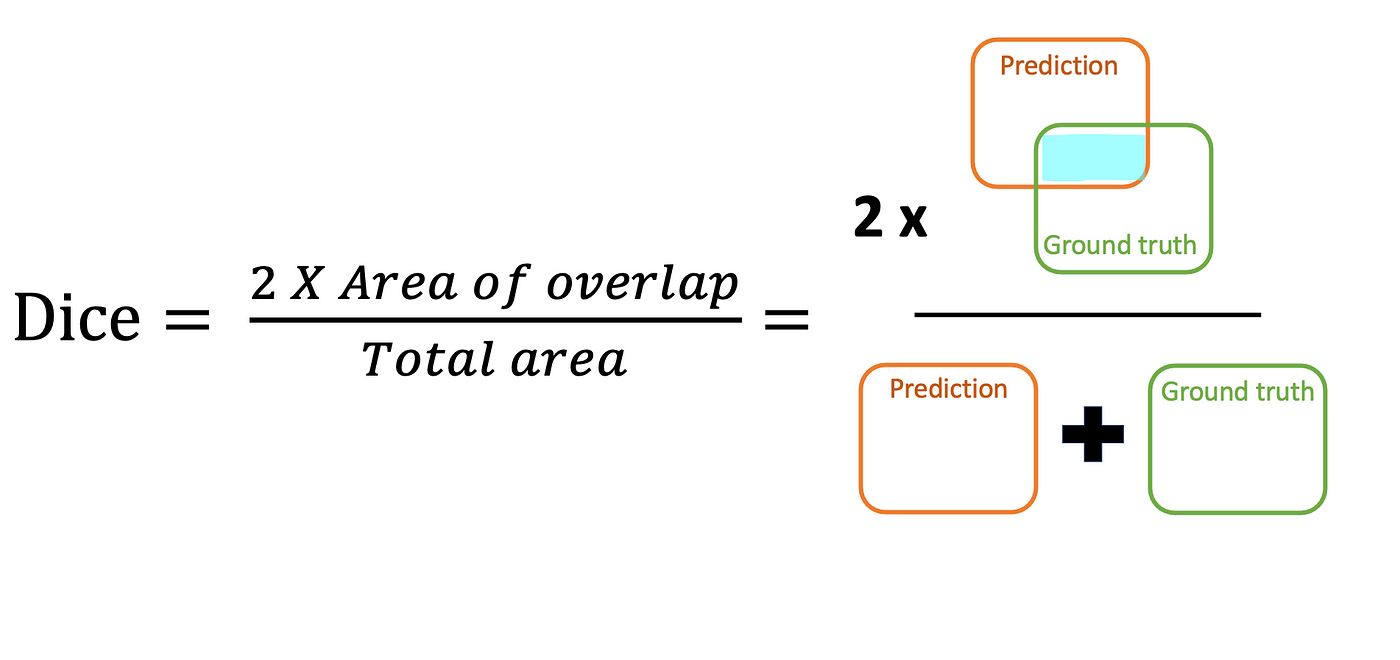
\includegraphics[width=0.7\columnwidth]{Immagini/dice_loss.png}
	\caption{Rappresentazione della Dice Loss}
	\label{fig:dice_loss}
\end{figure}

La Dice Loss è una metrica di perdita basata sul coefficiente di Dice, che è una
misura della somiglianza tra due campioni. È particolarmente utile per i dati
non bilanciati, come è spesso il caso nelle immagini mediche dove la regione di
interesse occupa una piccola parte dell'immagine. Il coefficiente di Dice è
definito dal' equazione \ref{eq:dice_loss}.

La \textit{Binary Cross-Entropy (BCE) Loss} è ampiamente usata nei problemi di classificazione
binaria, specialmente quando i dati di output sono probabilità che variano tra 0 e 1. Questa metrica
valuta quanto le predizioni del modello si discostino dai valori reali (etichette).

\begin{align}
	L & = L_{\text{Dice}} + L_{\text{BCE}}
	\label{eq:dice_bce_loss}
\end{align}

\begin{align}
	L_{\text{Dice}} & = 1 - \frac{2\sum_i^N p_i g_i + \varepsilon}{\sum_i^N p_i^2 + \sum_i^N g_i^2 + \varepsilon}
	\label{eq:dice_loss}
\end{align}

\begin{align}
	L_{\text{BCE}} & = -\frac{1}{N} \Bigg[ \sum_{i=1}^N g_i \log(p_i) + (1 - g_i) \log(1 - p_i) \Bigg]
	\label{eq:bce_loss}
\end{align}

Dunque, la \textit{loss} totale viene calcolata mediante:
\begin{align}
	L & = 1 - \frac{2\sum_i^N p_i g_i + \varepsilon}{\sum_i^N p_i^2 + \sum_i^N g_i^2 + \varepsilon} -\frac{1}{N} \Bigg[ \sum_{i=1}^N g_i \log(p_i) + (1 - g_i) \log(1 - p_i) \Bigg]
	\label{eq:dice_bce_loss_complete}
\end{align}
Dove:
\begin{itemize}
	\item $p_i$ rappresenta la probabilità predetta dal modello per il pixel $i$.
	\item $g_i$ è il valore di \textit{ground truth} per il pixel $i$.
\end{itemize}

\subsection{Intersection over Union(IoU)}
Per la metrica dell'accuratezza della segmentazione, è stata utilizzata la metrica \textit{Intersection over Union} (IoU),
poiché è una metrica che permette di valutare la capacità di segmentazione del modello
facendo il rapporto tra l'area di intersezione tra la maschera predetta e quella di \textit{ground truth} e l'area di unione tra le due maschere, formalmente:
\begin{align}
	\text{IoU} & = \frac{\text{TP}}{\text{TP} + \text{FP} + \text{FN}}
	\label{eq:iou}
\end{align}

Dove \textbf{TP} è il numero di \textit{True Positive}, \textbf{FP} è il numero
di \textit{False Positive} e \textbf{FN} è il numero di \textit{False
	Negative}.

\section{Validazione del Modello}
\label{sec:model_validation}

La \textit{cross-validation} (validazione incrociata) è un metodo essenziale nel machine learning
per valutare le prestazioni di un modello in modo robusto. Questa tecnica comporta la valutazione
del modello su più insiemi di dati per ottenere stime più affidabili delle sue capacità predittive,
contribuendo a mitigare il rischio di overfitting.

\begin{figure}[!ht]
	\centering
	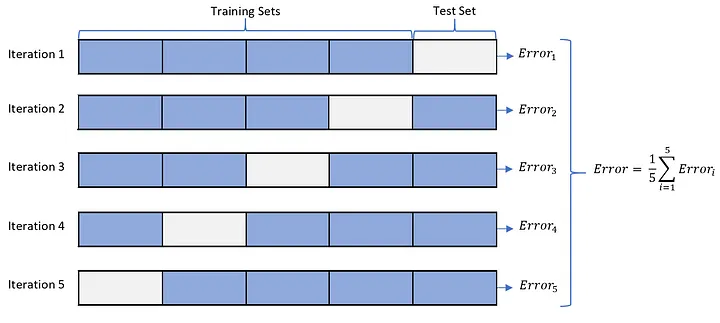
\includegraphics[width=0.7\textwidth]{Immagini/cross_validation.png}
	\caption{Rappresentazione grafica della Cross-validation}
	\label{fig:cross_validation}
\end{figure}

Fornisce stime più affidabili delle prestazioni del modello, riducendo il
rischio di ottenere stime di prestazioni spurie a causa di una singola
divisione dei dati.
